\documentclass[output=paper,modfonts,nonflat]{langsci/langscibook} 
\author{Archna Bhatia\affiliation{Florida Institute for Human and Machine Cognition, Ocala, FL, USA}\and Choh Man Teng\affiliation{Florida Institute for Human and Machine Cognition, Pensacola, FL, USA}\lastand James F. Allen\affiliation{University of Rochester, Rochester, NY, USA \\Florida Institute for Human and Machine Cognition, Pensacola, FL, USA} }
\title{Identifying senses of particles in verb-particle constructions}

\abstract{In order to attain broad coverage understanding, a system need not only identify multiword expressions such as verb-particle constructions\is{verb-particle construction} (VPCs), but must compute their meaning. It is not plausible to hand enumerate all possible combinations, although WordNet is an admirable start. This chapter focuses on the identification of senses of particles in VPCs in order to compute the meanings of VPCs -- using information obtained from existing lexical resources such as WordNet, and augmenting it with additional knowledge based on linguistic investigation of VPCs identified in terms of generalizations encoded in the TRIPS ontology. The approach consists of first determining compositionality of a VPC\is{verb-particle construction!compositionality} based on the information present in WordNet, and then assigning a relevant sense to the particle in a compositional VPC based on the sense classes\is{particle sense classes} we have identified and encoded in the TRIPS' computational lexicon. Contributions of the described work are twofold: (1) A discussion of senses of particles in VPCs and corresponding generalizations makes a linguistic contribution. (2) We show how linguistic knowledge can be used to automatically parse sentences containing VPCs and obtain a semantic representation of them.  An advantage of the described approach is that VPCs not explicitly found in lexica can be identified and semantically interpreted.\il{English}}

\begin{document}
\maketitle
\label{BHATIA-CHAPTER}





\section{Introduction } \label{bha:sec:intro}
To compute deep semantic representations of sentences\is{parsing!semantic}, we need to pay attention to the richness of lexical meaning. Multiword expressions (MWEs) constitute a significant proportion of the lexicon in any natural language \citep{Mor13}. In fact, \citet{Jac97} estimated the number of MWEs in a speaker's lexicon to be of the same order of magnitude as the number of single words. Thus, it is important to get a good interpretation of MWEs.

This chapter builds on and extends the work reported in \citet{Bha17} with focus on a specific type of MWEs, namely verb-particle constructions (VPCs)\is{verb-particle construction}. VPCs consist of a verb and an adverbial or prepositional particle, e.g., \ile{eat up}, \ile{fade out}, \ile{go on}, \ile{show off}, and \ile{walk down}.\footnote{Note that we focus on the particle usage here, not on the prepositional usage, i.e., a verb followed by a particle not a prepositional phrase. However, there may be an overlap in lexical semantic content (i.e., senses) of the homophonous particles and prepositions, see \sectref{sec:senses}.} Adding every single occurrence of such verb-particle combinations to a lexicon is not efficient nor ideal since knowledge about individual parts (verb and particle) can be leveraged for many of these VPCs as they are interpretable compositionally, e.g., \ile{fly up}. 

Other VPCs that indeed are noncompositional\is{non-compositionality} require special interpretation, and hence need to be added into the lexicon, e.g., \ile{bring off} `achieve a goal' and \ile{egg on} `urge someone for an action that might not be a good idea'. Our work on compositionality of VPCs\is{verb-particle construction!compositionality}, described in \citet{Bha17} and developed further here, helps identify VPCs of each type for a proper treatment.

For an inventory of senses for verbs, many lexical resources, such as WordNet \citep{Mil95,Fel98} and the TRIPS lexicon \citep{All17}, are available that can be leveraged for interpreting compositional VPC types. In contrast, there is not much for particles except for a few attempts at the semantics of a few particles, such as \ile{up} \citep{Coo06} and \ile{out} \citep{Tyl03}. However, particles seem to add their own semantics in compositional VPCs and are found to be regular when occurring with verbs in specific verb classes. For example, the particle \ile{up} has a DIRECTION sense\is{particle sense classes!direction} when it appears in resultative VPCs with verbs of motion, such as \ile{wander/stroll/go/run up} \citep{Vil06}. In this chapter, we provide a refined set of senses for particles in VPCs originally presented in \citet{Bha17}. We discuss and demonstrate how these senses are identified in compositional VPCs in order to compute meanings of sentences containing VPCs. 

For computation of meaning, we use a broad coverage deep semantic parser, TRIPS \citep{All07}, which combines semantic, ontological, and grammatical information to produce semantic representations\is{parsing!semantic}.\footnote{For a more detailed overview of the TRIPS system, refer to \citet{All17} and \citet{All08}.\\The TRIPS parser can be accessed at: \url{http://trips.ihmc.us/parser/cgi/parse}} We encode the semantics of particles mentioned above in the TRIPS ontology.\footnote{The TRIPS ontology can be accessed at: \url{http://www.cs.rochester.edu/research/cisd/projects/trips/lexicon/browse-ont-lex-ajax.html}} The ontology encodes semantic types, the set of word senses and semantic relations that can be used in logical form (LF) graphs. Word senses are defined based on subcategorization patterns and selectional restrictions driven by linguistic considerations. The semantic types in the ontology are, to a large extent, compatible with FrameNet \citep{Joh00}. The ontology uses a rich set of semantic features. Unlike WordNet, our ontology does not attempt to capture all possible word senses, but rather focuses on the level of abstraction that affects linguistic processing.

This chapter builds on the work described in \citet{Bha17} in the following ways: Improvements have been made in the classification of compositionality and sense types as well as in the heuristics to automatically identify the types. The evaluation is made more robust with a larger test data set with full coverage of the heuristics\is{verb-particle construction!heuristics for compositionality}. A more thorough analysis has led to the identification of generalizations regarding sense types. 

%The description of the \isi{compositionality} types has been revised. The sense types have also been revised. In order to determine the \isi{compositionality} categories and the sense categories, specific tests have been identified as shown in \figref{fig:tests} and \figref{fig:tests-senses}. The \isi{\is{heuristics} for compositionality} of VPCs have been modified. Also, the \isi{heuristics} now have full coverage, i.e., each VPC is assigned a \isi{compositionality} label. For the evaluation of the \isi{heuristics}, the number of test VPCs has been doubled in the original test set (Test Set 1). Also, another test set (Test Set 2) has been created and used to test \isi{heuristics} 1 and 2 which were not evaluated previously in \citet{Bha17}. The revised evaluation is presented in \tabref{tab:1:eval-heur}, where our definitions of the evaluation categories (precision and coverage) have also been provided. Manual annotations for \isi{compositionality} types and senses with a more detailed analysis is performed and presented. Generalizations regarding each sense type are identified and presented in \tabref{tab:1:senseclasses-prtcls} and \tabref{tab:1:findings-prtcls} which are encoded in the TRIPS ontology. These generalizations are used to identify senses of particles. Additionally, a discussion of the procedure to compute semantics of sentences involving VPCs using TRIPS logical forms is presented using three example sentences involving VPCs with different senses for the particle up.

The chapter is organized as follows: Previous work on VPCs is discussed in \sectref{sec:prevwork}. A classification of VPCs based on their compositionality\is{verb-particle construction!compositionality} is discussed in \sectref{sec:classification} with its feasibility using \isi{inter-annotator agreement} in \sectref{sec:iaa-comp}. A set of heuristics\is{verb-particle construction!heuristics for compositionality} to identify different classes of VPCs are presented in \sectref{sec:heuristics} and their evaluation in \sectref{sec:eval}. In \sectref{sec:prtcl-semcs}, we discuss the semantics of particles in VPCs. An inventory of general sense classes\is{particle sense classes} for particles used in VPCs is provided in \sectref{sec:senses}, which is followed by a brief discussion of manual sense annotations as well as the use of compositionality heuristics\is{verb-particle construction!heuristics for compositionality} for sense identification. In \sectref{sec:generalizations}, we present various generalizations corresponding to the identified sense classes\is{particle sense classes} for the particles, and briefly discuss how a computational lexicon (including a lexicon for particles) is built for the computation of meaning for VPCs. Through examples, we demonstrate the general procedure to compute the meaning of sentences involving compositional VPCs and that the linguistic generalizations are reasonably helpful in the accurate identification of particle senses\is{particle sense classes} in VPCs. \sectref{bha:sec:conclusions} concludes the chapter.

\section{Related work} \label{sec:prevwork}
A lot of computational literature on VPCs focuses on the identification or extraction of VPCs, or on the compositionality of VPCs\is{verb-particle construction!compositionality}, as discussed below. There are a few articles dealing with different senses of particles\is{particle sense classes}, but they usually focus on only one or two specific particles rather than on a broader coverage of particles. For example, \citet{Nii14} discusses grammaticalization of the particle \ile{away} in English, specifying directional, completive, and continuing or iterative usages of the particle. \citet{Ish10,Ish12} also studies grammaticalization of the particle \ile{away} together with the particle \ile{out}, presenting a classification\is{verb-particle construction!classification} of VPCs into three categories of fully compositional, partially idiomatic, and fully (or highly) idiomatic. 

\citet{wiki50} presents the Wiki50 corpus that has 446 VPCs (342 unique types) annotated. \citet{Ban02} makes an attempt to identify different types of VPCs in terms of compositionality\is{verb-particle construction!compositionality} and builds a (decision tree) classifier to identify the four types. \citet{Ban03} also adopt a similar approach for compositionality. As an annotation experiment, they investigate various VPCs to see whether the sense is contributed by the verb and/or the particle. They build four classifiers for automatic semantic analysis of VPCs. \citet{Pat04} also have a similar approach, but they focus on automatic classification\is{verb-particle construction!classification} of different types of compositionality. Unlike our work, in all these works, the focus is on compositionality only, not on the identification of actual senses of the particles.

\citet{Coo06} discuss various senses for the particle \ile{up}\is{particle sense classes} in a cognitive grammar framework, annotate a dataset and perform some classification\is{verb-particle construction!classification} experiments to identify the senses of \ile{up} in unseen data. As a linguistic study, \citet{Jac02} provides a very nice discussion of various types of VPCs involving particles such as directional particles, aspectual particles, time-AWAY constructions, and some idiomatic constructions. Our work differs from theirs in having a broader coverage of particles and/or strong emphasis on ontology with respect to the sense classes of the particles and how different \isi{particle sense classes} relate to verbal ontological classes.

\citet{Fra76} mentions semantic properties of verbs affecting patterns of verb-particle combinations, for instance semantically similar verbs \ile{bolt/cement/clam{\slash}glue/paste/nail} all can combine with the particle \ile{down} and specify the objects that can be used to join material. Our approach is based on the similar assumption that there are generalizations, such as particles with certain sense classes combine with specific verb classes or ontological classes. \citet{Vil03} also adopts the same approach where she tries to encode the information in terms of lexical rules and restrictions, etc. However, her focus is on obtaining productive patterns in VPCs rather than on their interpretation.

Our work also differs from the previous work mentioned above in the following respect: We emphasize the building of complete semantic representations of the sentences, not just the particles' semantics or just the classification of VPCs\is{verb-particle construction!classification}. Similar to our criteria for compositionality, \citet{McC03}, \citet{Bal03}, and \citet{Ban03} have looked at \isi{distributional similarity} as a measure of compositionality of VPCs\is{verb-particle construction!compositionality}. In contrast to the approaches focusing on statistical classification based on word/syntax features, our approach (both symbolic and statistical) uses information obtained from existing lexical resources, such as WordNet, for the classification of VPCs. We augment it with additional knowledge based on the linguistic investigation of VPCs identified in terms of generalizations, which we encode into an ontology, in order to compute the semantics of the compositional classes.


\section{Classification of VPCs} \label{sec:classification}

VPCs\is{verb-particle construction} have often been classified in terms of their compositionality\is{verb-particle construction!compositionality} (i.e., whether all constituents of a VPC, the verb and the particle, contribute their simplex meanings to the overall semantic content of the VPC). The classes fall somewhere between fully compositional VPCs, e.g., \ile{fly up}, and fully idiomatic VPCs, e.g., \ile{egg on}. For example, see \citet{Fra76}, \citet{Che86}, \citet{Odo98}, \citet{Deh02}, and \citet{Jac02}.

We also classify VPCs into two types\is{verb-particle construction!classification}, compositional VPCs and noncompositional VPCs. The difference between the two classes is that the meaning of a compositional VPC is the sum of the meanings of its parts (the verb and the particle) whereas a noncompositional VPC\is{non-compositionality} %may have (additional) 
has semantic content which is not contributed by the individual constituents (i.e., the verb and the particle). 

The compositional VPCs can be further classified into three subtypes: symmetrically compositional VPCs, light particle compositional VPCs (LP-compositional VPCs), and light verb compositional VPCs (LV-compositional VPCs), based on the type of semantic content contributed by each of the constituents. Symmetrically compositional VPCs refer to VPCs in which both constituents, the verb and the particle, contribute their simplex meanings (their lexical-semantic content). For example, in \ile{Debris \lex{flew up} and hit the window in the furthest unit}, the senses for the verb \ile{fly} (e.g., in WordNet, sense fly\%2:38:00) as well as the particle \ile{up} (e.g., in WordNet, sense up\%4:02:00) combine together to provide the meaning of the VPC \ile{fly up}.\footnote{For this study, we have used WordNet version 3.0. The numbers appearing after the symbol \% in the WordNet senses represent the sense keys in WordNet.} We distinguish the other two compositional VPC types from the symmetrically compositional VPCs only in the aspect that in the other two types, the particle or the verb have a relatively lighter contribution than the other constituent which adds its regular lexical-semantic content.\footnote{The term ``light particle" is used in analogy with the term ``light verb" which is commonly used in the literature for verbs with bleached content.} 

LP-compositional VPCs\is{verb-particle construction}\is{verb-particle construction!classification}\is{verb-particle construction!compositionality} involve particles which, instead of contributing a pre\-position like lexical-semantic content, contribute aspectual information to the VPCs. Verbs contribute most of the lexical-semantic content in such VPCs. For example, in \ile{Susan \lex{finished up} her paper} \citep{Ban03b}, the verb \ile{finish} contributes its regular lexical content (e.g., in WordNet, sense finish\%2:30:02). However, the particle \ile{up}, instead of contributing its regular lexical-semantic content, adds aspectual information that the action was completed (i.e., the COMPLETELY sense in our sense inventory)\is{particle sense classes!completely}. See \sectref{sec:senses} for the specific senses of particles. 

LV-compositional VPCs\is{verb-particle construction} involve light verbs which carry bleached meaning compared to regular verbs, e.g., CAUSE and BECOME. The particles contribute their regular lexical-semantic content to the VPCs's semantics.  For example, in \ile{The thief \lex{made away} with the cash}, the particle \ile{away} contributes its regular meaning (e.g., WordNet sense away\%4:02:00), but the verb \ile{make}, instead of contributing its regular meaning (e.g., WordNet sense make\%2:36:01), adds a bleached meaning (e.g., cause to be). For details on the procedure to compute meanings of sentences with compositional VPCs, see \sectref{sec:generalizations}.

In a noncompositional VPC\is{non-compositionality}, the sum of meanings of individual parts (the verb and the particle) may not completely account for the meaning of the VPC or may not account for it at all. Let's consider a few examples. In \ile{They \textbf{turned away} hundreds of fans}, the VPC \ile{\textbf{turned away}} is noncompositional  despite the fact that the individual constituents' semantic content is reflected in the semantics of the VPC, since the VPC has additional content (`refuse entrance or membership') besides those contributed by the constituents. This additional content is not inferable from the individual parts and needs to be included in the lexical entry for the VPC. Another example of a noncompositional VPC is idiomatic usages. For example, the VPC \ile{\lex{egged on}} in \ile{John wouldn't have done the dangerous experiment if his brother hadn't \lex{egged} him \lex{on}} involves idiosyncratic content that is not inferable from the parts and hence needs to be encoded in the lexicon. Some idiomatic usages may involve certain generalizations which may aid in interpretation of the VPC. For example, two generalizations regarding the interpretation of the noncompositional VPC \ile{\lex{take up}} are (i) it takes the sense `starting to do an activity' when it appears with activities as direct objects, e.g., \ile{She \lex{took up} photography/swimming} [activities] and (ii) it takes the sense `assume a responsibility' when it appears with positions/responsibilities as direct objects, e.g., \ile{She \lex{took up} her position} [responsibility/position]. 

For identification of the compositionality type for a given VPC\is{verb-particle construction!compositionality}, one may adopt tests as in \figref{fig:tests}.

\begin{figure}
%\vspace*{-1mm}
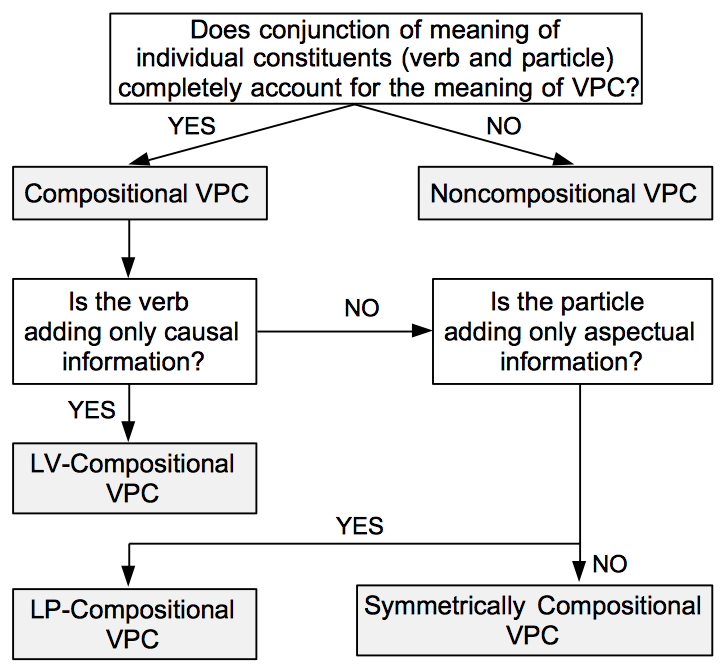
\includegraphics[width=.66\textwidth]{figures/block_compositionality_mod7}
%\vspace*{-2mm}
\caption{Tests to identify compositionality type}\label{fig:tests}
\end{figure}
%\vspace*{-4mm}

\subsection{Human agreement on coarse-grained classification of VPCs} \label{sec:iaa-comp}

From among all the VPCs\is{verb-particle construction} for which WordNet has an entry, we automatically extracted 50 random VPCs such that four particles, namely \ile{up}, \ile{down}, \ile{out}, and \ile{away}, were represented in the extracted VPCs.\is{verb-particle construction!classification}\is{inter-annotator agreement} Since a VPC may have both compositional and noncompositional usages\is{non-compositionality} in different contexts (represented by different word senses or synsets in WordNet), we restricted the assignment of annotation label for a specific VPC to only one label by considering a single synset from WordNet for annotations. Some of the WordNet synsets do not have an example with the exact VPCs.\footnote{It may have examples which use related verbs or related VPCs instead, or it may not have an example at all. For example, the WordNet entry \ile{turn\_away\%2:38:02} for the VPC \ile{\lex{turn away}} does not have any example with the VPC itself.} We restricted the automatic extraction of VPCs to only those VPCs for which WordNet had a synset which included the VPC in its example. This synset was presented to the annotators together with the VPC to be annotated and the example usage.

These test VPCs were manually annotated by three annotators for compositionality labels\is{verb-particle construction!compositionality}. Fleiss' kappa score \citep{Fle71} was used to test inter-annotator reliability. The three sets of annotations achieved a score of 0.651, an intermediate-good score.\footnote{NLTK's agreement package was used to calculate the Fleiss' kappa score which showed intermediate-good agreement. Cohen's kappa score \citep{Coh60} was also calculated using the same package showing substantial agreement, also with a score of 0.651.} We also created the gold annotations from the three sets of manual annotations. In cases of disagreement, the three annotators discussed reasons for their decisions and arrived at a consensus to create the gold annotations for the VPCs. The distribution of compositional vs. noncompositional VPCs in the automatically extracted 50 test VPCs was $60\%$ vs. $40\%$. In terms of the specific compositionality types, the distribution was $30\%$ for symmetrically compositional cases, $30\%$ for LP-compositional, and $40\%$ for noncompositional cases\is{non-compositionality}. Note that the 50 randomly extracted test VPCs did not have an instance of an LV-compositional VPC.

In the manual annotations, there were 37 VPCs out of 50 for which there was full agreement among all three annotators on the coarse-grained labels for compositionality type. Since there were only two coarse-grained labels (compositional and noncompositional), for the rest of the 13 VPCs, there was agreement between two out of three annotators for the compositionality label. The annotators disagreed more on the compositional cases ($76.92\%$ of the disagreements were on the compositional VPCs) than on the noncompositional ones ($23.08\%$).

In terms of VPCs with certain particles, VPCs with the particle \ile{down} were found to be the most challenging for the annotators. For $42.86\%$ of the usages of VPCs with \ile{down} (3 out of 7 usages) among the 50 test cases, the annotators did not agree on the annotation label. On the other hand, VPCs with the particle \ile{up} were found to be the least challenging. For only $14.29\%$ of the cases (3 out of 21 usages), the annotators disagreed on the compositionality type. This may be due to the fact that VPCs with the particle \ile{up} have a higher frequency than VPCs with other particles \citep{Vil06}, such as \ile{down}, and hence users have relatively better intuitions about VPCs with the particle \ile{up} compared to VPCs with the particle \ile{down}.


\subsection{Heuristics for compositionality of VPCs} \label{sec:heuristics}

As a first step toward an interpretation of VPCs, we need to determine whether a given VPC is compositional or not.\is{verb-particle construction!heuristics for compositionality} To perform this task automatically, we employ a number of heuristics that make use of the rich inventory of hierarchically organized word senses (i.e., synsets) in WordNet which contains over 100,000 words including 64,188 multiwords. Heuristics 1--6 below are used to identify compositional VPCs, whereas heuristic 7 indicates non-compositionality.

\begin{enumerate}
\setlength\itemsep{0em}
\item If the verb is among the list of light verbs, and WordNet does not have an entry for the VPC, it is LV-compositional. For example, the VPC \ile{make away} uses the light verb \ile{make} and the VPC does not have an entry in WordNet.

\item Given a VPC, if heuristic 1 does not apply and WordNet has an entry for the verb as well as for the particle, but no entry for the VPC, VPC is compositional (LP-compositional or symmetrically compositional). For example, \ile{fly} with the sense key fly\%2:38:01 as well as \ile{up} with the sense key up\%4:02:00 appears in WordNet, but \ile{fly up} does not appear in any synset in WordNet.

\item If WordNet has the VPC as well as the verb in the same synset, VPC is LP-compositional. For example, the VPC \ile{sort out} (sort\_out\%2:31:00) and the verb \ile{sort} (sort\%2:31:00) both appear in the same synset in WordNet.


\item 
\sloppy 
If WordNet has the verb in the VPC as a hypernym for the VPC, VPC is either symmetrically compositional or LP-compositional. For example, compositional VPC \ile{push up} (push\_up\%2:38:00) has the verb \ile{push} (push\%2:38:00) as its direct hypernym.

\item If WordNet has the verb in the definition (in its base or inflected form) of the synset where the VPC appears, the VPC is either symmetrically compositional or LP-compositional. For example, the compositional VPC \ile{move up} (move\_up\%2:38:00) has the verb \ile{move} in its definition \ile{move upwards}.

\item If WordNet has the relevant VPC as well as another VPC with the verb replaced with another verb in the same synset, the VPC is compositional (either symmetrically compositional or LP-compositional or LV-compositional). For example, the compositional VPCs \ile{pull out} (pull\_out\%2:35:00) and \ile{rip out} (rip\_out\%2:35:00) appear in the same WordNet synset.

\fussy
\newpage 
\item If none of the above heuristics apply, the VPC is noncompositional\is{non-compositionality}. For example, none of the above heuristics apply to the idiomatic VPC \ile{catch up} (catch\_up\%2:38:0).

\end{enumerate}


\subsection{An evaluation of the heuristics for compositionality of VPCs} \label{sec:eval}

For an evaluation of the heuristics\is{verb-particle construction!heuristics for compositionality}, we used two test sets: (i) Test Set 1: the test set consisting of the same 50 randomly extracted VPCs that were used to calculate \isi{inter-annotator agreement} scores mentioned in \sectref{sec:iaa-comp}, and (ii) Test Set 2: a test set consisting of 653 VPCs created using the VPCs on the first page of each of the four English wiktionary entries with the title ``Category: English phrasal verbs with particle" for particles \ile{up}, \ile{out}, \ile{down}, and \ile{away} respectively.\is{verb-particle construction!heuristics for compositionality}

A Python implementation of the heuristics was applied to the test VPCs in both test sets to assign them a compositionality label. Heuristics 1--6 identify compositional VPCs, whereas heuristic 7 identifies noncompositional VPCs\is{non-compositionality}. Note that together these heuristics have full coverage, i.e., a prediction is made for each of the VPCs in the test sets. Heuristics 1 and 2 apply to VPCs for which WordNet does not have an entry.  Heuristics 3-6 apply to VPCs for which WordNet has an entry. Heuristic 7 applies when none of the heuristics 1-6 apply.

Since Test Set 1 consisted of VPCs that were randomly extracted from WordNet, only heuristics 3--7 could be evaluated on Test Set 1. Heuristics 1 and 2 could not be evaluated using this test set since these two heuristics apply to VPCs that are not included in WordNet. In order to test heuristics 1 and 2, we used Test Set 2 which has VPCs that may or may not be included in WordNet. 

Test Set 1 has manually created gold annotations. Hence, the labels assigned by the heuristics were tested against them 
for the VPCs in Test Set 1. For Test Set 2, on the other hand, we examined the heuristics-assigned labels corresponding to heuristics 1 and 2 manually. 
 

An evaluation of the heuristics on Test Set 1 is presented in \tabref{tab:1:eval-heur}. Heuristics 3, 4, and 5 (used to identify compositional VPCs) performed perfectly in identifying compositionality of VPCs whereas heuristic 6 (also intended to identify compositional VPCs) did not have as high precision. Two out of the three cases where heuristic 6 made an incorrect prediction, however, involved noncompositional VPCs\is{non-compositionality} for which the individual constituents' meaning was also reflected in the semantics of the VPCs even though they also had additional content that was not inferable based on the constituents alone. The fact that the constituents' semantics was reflected in the VPCs' semantics was what heuristic 6 had captured. Heuristic 7 (the only heuristic used to identify noncompositional VPCs) also had a lower but better than chance performance in comparison to the other heuristics. 


\begin{table}
\caption[Evaluation of heuristics 3--7 using Test Set 1 (50 test cases)]{Evaluation of heuristics 3--7 using Test Set 1 (50 test cases)\footnote{We define precision as Cn/Tn and coverage as Tn/N, where N is the corpus size, Tn is the sample size that heuristic n is applicable to, and Cn is the number of correct assignments it makes.}}
\label{tab:1:eval-heur}
%\vspace*{-2mm} 
 \begin{tabularx}{\textwidth}{YYY}
  \lsptoprule
    Heuristic \# & Precision for the heuristic ($\%$)  & Coverage of the heuristic ($\%$)\\ 
  \midrule
  3 & 100 & 16 \\
  4 & 100 & 6 \\
  5 & 100 & 12 \\
  6 & 76.92 & 26 \\
  7 & 58.62 & 58 \\
  \midrule 
   Overall (heuristics 3--7) & 70 & 100 \\
  \lspbottomrule
 \end{tabularx}
\end{table}


Overall, heuristics 3--7 had a precision of $70\%$ in assigning a label (compositional or noncompositional) to a VPC. Whenever multiple heuristics applied to a VPC (14\% of the test cases), they were always correct in their prediction. This suggests that presence of multiple characteristics of compositionality (represented by the heuristics) may be a reliable indicator of compositionality. In 86\% of the cases, a single heuristic identified the VPC as representative of its own category (compositional or noncompositional). Regarding the relatively lower performance of heuristic 7, since noncompositonal VPCs carry additional information not contributed by individual constituents (common sense knowledge or idiosyncratic information), it may not be observable and hence is not captured using a heuristic as easily or directly.

More investigation is required into heuristics 6 and 7 to see how they can be modified to make them better usable for identification of the compositionality type of a VPC. For example, a future step may be to examine if certain generalizations exist in terms of verb types and particle types that can help us further determine when the cases identified by these heuristics are compositional or noncompositional.\is{non-compositionality}

As a result of the examination of the heuristics' output\is{verb-particle construction!heuristics for compositionality}, we noticed a few more indicators which could also be incorporated into the heuristics to %increase their coverage 
improve their performance in the future. For example, if the word \ile{completely} or \ile{thoroughly} appears in the definition of a synset of a VPC, the particle in the VPC may carry the aspectual sense COMPLETELY\is{particle sense classes!completely}. Hence, it could be labelled as a compositional VPC (specifically, as an LP-compositional VPC).

As mentioned above, for an evaluation of the heuristics 1 and 2, we used Test Set 2 that consisted of 653 VPCs, a subset of the VPCs mentioned in the English wiktionary. The Python implementation of the heuristics mentioned above was used to assign compositionality labels to the VPCs in Test Set 2. Out of the 653 VPCs, heuristic 1 applied to only 2 VPCs ($0.3\%$ of the test items) and heuristic 2 applied to 280 VPCs ($42.88\%$ of the test items). Heuristic 7 applied to 9 other VPCs that did not have a WordNet entry. Overall, $44.56\%$ of the test cases did not have an entry in WordNet.  Heuristic 2 covered $96.22\%$ of these cases with reasonable precision ($80\%$, evaluated on 15 randomly selected test VPCs to which heuristic 2 applied).

Next, we move on to the semantics of particles in VPCs. We will focus mostly on the compositional VPCs for the rest of this chapter. 

\section{Semantics of particles in VPCs} \label{sec:prtcl-semcs}

As mentioned in \sectref{sec:classification}, particles contribute to the overall semantics of compositional VPCs. In order to study the contribution of particles in VPCs, in our prior work \citep{Bha17}, we conducted an investigation of VPCs consisting of verbs in the ontology class ONT::EVENT-OF-CAUSATION in the TRIPS ontology. This class consisted of 1383 words with verb senses (and a total of 1784 verb senses of those words). Our investigation consisted of combinations of these verbs with the following particles (wherever the combinations %were possible 
appeared as VPCs): \ile{across}, \ile{away}, \ile{by}, \ile{down}, \ile{in}, \ile{into}, \ile{off}, \ile{on}, \ile{out}, \ile{over}, \ile{through}, and \ile{up}.\footnote{While we do find prepositional phrasal verb constructions with \ile{into}, we did not find any VPCs involving intransitive usages of \ile{into}.} We searched for examples for each of the combinations using Google and manually went through each of the examples to check for a number of properties. For example, we checked if any of the verb or the particle contributed to the overall meaning of the VPC. We identified the senses particles had in the VPCs if any. We checked: (i) if the particle could be taken out without a major change in the meaning, (ii) if the particle expressed RESULT or could be replaced with a RESULT-Prepositional Phrase,\footnote{RESULT is one of the argument roles identified in the TRIPS ontology. The argument roles signal different argument positions for predicates as well as have their own inferential import, some other examples are AGENT, AFFECTED, MANNER, LOCATION, and FIGURE.} (iii) if a corresponding VPC consisting of the particle with the opposite polarity was also possible (e.g., \ile{take in} vs. \ile{take out}), (iv) if specific argument types (e.g., MANNER, RESULT, LOCATION, AFFECTED) were instantiated in the sentence, etc. In the rest of this section, we present the sense classes particles in compositional VPCs tend to fall into. 

\subsection{Sense classes for particles in VPCs} \label{sec:senses}

While particles may encode subtle nuances of meanings in each of their occurrences in (compositional) VPCs, they may also display some general senses across many VPCs. WordNet attempts to capture the nuances by storing each of the VPCs as a separate lexical item. However, this approach results in having as many sense categories as there are VPCs and we lose information about the common contributions made by the particles in VPC semantics which can be useful while producing semantic representation of sentences with new VPCs not stored in WordNet or another lexical resource. Hence, we focus on the general senses particles display across compositional VPCs.\is{particle sense classes} 

We identified two general sense classes for the particles in compositional VPCs, namely DIRECTION and ASPECTUAL\is{particle sense classes!aspectual}. The DIRECTION sense class has a number of subclasses, each instantiated by a specific directional particle, such as \ile{away}, \ile{down}, \ile{in}, \ile{off}, \ile{on}, \ile{out}, and \ile{up} denoting a specific direction sense. For example, the directional particle \ile{away} instantiates the subclass DIRECTION-AWAY\is{particle sense classes!direction-away} in \ile{I took one last look at the house and \textbf{walked away}}. Similarly, the particle \ile{out} in \ile{My mom never \textbf{threw} it \textbf{out}} and the particle \ile{up} in \ile{The magic ketchup should sink when you squeeze the bottle and \textbf{float up} when you release it} instantiate subclasses DIRECTION-OUT\is{particle sense classes!direction-out} and DIRECTION-UP\is{particle sense classes!direction-up} respectively. The DIRECTION sense class particles assume the RESULT role in relation to the verb. For example, in the DIRECTION-AWAY example, the particle \ile{away} denotes the RESULT of a \ile{walking} event in terms of the direction the AFFECTED entity is walking to.

The ASPECTUAL sense class\is{particle sense classes!aspectual} has two subclasses, namely COMPLETELY\is{particle sense classes!completely} and CONTINUING\is{particle sense classes!continuing}, where the particle modifies the verb by providing aspectual information. In terms of the TRIPS semantic roles, the aspectual sense particles assume the MANNER role in relation to the verb. The COMPLETELY sense is used to express that the activity denoted by the verb is performed to the full extent or with thoroughness. Particles with COMPLETELY sense may also emphasize the telicity of an action. For example, the particle \ile{out} in \ile{He \textbf{sorted out} every scrap of manuscript, every map, and the native letters} emphasizes that each of the items mentioned were thoroughly and completely sorted. Particles \ile{up}, \ile{out}, and \ile{down} are used more often than other particles to convey this aspectual sense.

\newpage 
The CONTINUING sense\is{particle sense classes!continuing} is used to emphasize the durative nature of the event denoted by the verb. For example, in \ile{Day after day she \textbf{worked away} ...} the particle \ile{away} conveys that the activity continued for a duration. The particles in this class may also convey an iterative sense when they are used with semelfactive verbs, e.g., note the use of the particle \ile{away} in \ile{Start your explorations here, \textbf{click away} all you want}. Usually particles \ile{away} and \ile{on} are used to convey this sense in VPCs.

These sense classes correspond to the VPC classes based on their compositionality types mentioned in \sectref{sec:classification}. For example, the DIRECTION sense class\is{particle sense classes!direction} is generally instantiated by the symmetrically compositional or LV-compositional VPCs. The ASPECTUAL sense class\is{particle sense classes!aspectual}, on the other hand, is instantiated by the LP-compositional VPCs. Besides these two sense classes, there are a few other senses that particles may express in VPCs corresponding to the symmetrically compositional and LV-compositional VPCs. For example, the senses IN-WORKING-ORDER-VAL\is{particle sense classes!in-working-order-val} and NOT-IN-WORKING-ORDER-VAL\is{particle sense classes!not-in-working-order-val} mentioned in \tabref{tab:1:senseclasses-prtcls} and \tabref{tab:1:findings-prtcls-3senses} are expressed by particles in LV-compositional VPCs. These senses are usually conveyed by the particles \ile{up}, \ile{down}, and \ile{out}. Similarly, the sense DISAPPEARANCE\is{particle sense classes!disappearance}, conveyed by the particle \ile{away}, may be taken to correspond to the particle %particles 
in symmetrically compositional VPCs. %This sense is conveyed by the particle \ile{away}. 
\tabref{tab:1:senseclasses-prtcls} contains information about each of these senses and corresponding sense classes for the particles \ile{up}, \ile{down}, \ile{away}, and \ile{out}. \tabref{tab:1:findings-prtcls-sense-classes} and \tabref{tab:1:findings-prtcls-3senses} present generalizations corresponding to these senses and sense classes. 


\begin{comment}
\begin{table}\Large
\caption{Observations about senses of particles \ile{up}, \textit{down}, \textit{away} and \textit{out} in compositional VPCs. Note that NP* refers to the object argument of a transitive verb, e.g., \textit{the carpet} in \textit{he took the carpet up}, or the subject of an intransitive verb, e.g., \textit{he} in \textit{he skied down}.}
\label{tab:1:findings-prtcls}
\vspace*{-2mm}
\scalebox{0.38}{
 \begin{tabular}{p{1.5in}p{0.5in}p{2.6in}p{1.7in}p{5.6in}}
  \lsptoprule
   \textbf{Sense class}: \newline Sense type
        & Prtcl
        & Example
        & Verb ontology type
        & Generalizations\\
    \midrule
  \textbf{DIRECTION}: \newline DIRECTION-UP, DIRECTION-DOWN, DIRECTION-AWAY, DIRECTION-OUT
    & up, down, away, out
    & He took the carpet up. \newline He skied down. \newline He ran away. \newline He cried out.
    & motion, \newline movement-related verbs
    & verb trajectory = + \newline Particle relative to some scale/domain \newline PP alternative is possible for the particles \textit{up}, \textit{down}, and \textit{out}. \newline The particle \textit{away} can take a PP-location as its GROUND argument. \newline Cases pass two tests: (1) Is there a change in physical location/on a scale? (2) Does the entity exist anywhere? \newline DIRECTION-UP is also possible with verbs in the TRIPS ontology classes apply-force and acquire.\newline DIRECTION-DOWN is also possible with verbs in the TRIPS ontology classes hitting.\newline DIRECTION-AWAY is also possible with event-of-change verbs where grammatical resultative construction is used. \newline DIRECTION-OUT is also possible with verbs of vocalization (and the verbs in the TRIPS ontology classes locution and manner-say) and some perception verbs. \\\\
  \textbf{ASPECTUAL}: \newline COMPLETELY
    & up, down, out
    & Clean up the room! \newline London nightclub closed down over fights with knives and bottles. \newline He sorted out every scrap of manuscript, every map, and the native letters.
    & event-of-change 
    & verb trajectory = - \newline PP alternative not possible \newline Default sense with event-of-change verbs \newline COMPLETELY for the particle \textit{up} is also possible with verbs in the TRIPS ontology classes protecting, joining, acquire-by-action, herd and arrange-text.\newline COMPLETELY for the particle \textit{down} is also possible with verbs in the TRIPS ontology classes change, consume, protecting, put and pursue. \newline COMPLETELY for the particle \textit{out} is also possible with verbs in the TRIPS ontology classes evoke-tiredness, arranging and put.\\\\
  \textbf{ASPECTUAL}: \newline CONTINUING
    & away
    & Night and day they hammered away, \newline coming on like great waves. \newline He scrubbed away at the floor.
    & event-of-action 
    & verb trajectory = - \newline Usually with atelic verbs \newline Iterative usage with semelfactive verbs \newline PP alternative not possible, i.e., particle cannot take NP object, \newline but can take PP object in conative constructions \newline CONTINUING is also possible with verbs in the TRIPS ontology class event-of-action.\\\\ 
  IN-WORKING-ORDER-VAL
    & up
    & Bring the browser up! 
    & light/causal verbs 
    & NP* is phys-obj \newline object-function = provides-service-up-down \newline i.e., the entity is a device with some functionality \newline PP alternative not possible\\\\
  NOT-IN-WORKING-ORDER-VAL
    & down, out 
    & The computer went down again. \newline The national electric grid went out.
    & light/causal verbs
    & NP* is phys-obj \newline object-function = provides-service-up-down \newline i.e., the entity is a device with some functionality. \newline PP alternative not possible \newline NOT-IN-WORKING-ORDER-VAL is also possible for the particle \textit{down} with verbs in the TRIPS ontology class event-of-undergoing-action.\\\\ 
  DISAPPEARANCE
    & away
    & The echo died away.\newline The music faded away.
    & verbs of disappearing
    & verb trajectory = - \newline Usually with verbs of disappearance \newline PP alternative not possible \newline Cases fail two tests: (1) Is there a change in physical location/on a scale? (2) Does the entity exist anywhere? \newline DISAPPEARANCE is also possible with verbs in the TRIPS ontology classes event-of-undergoing-action and change.\\
  \lspbottomrule
 \end{tabular}}
\end{table}
\end{comment}

 
\begin{table}%\LARGE
\caption{Sense classes for particles \ile{up}, \ile{down}, \ile{away}, and \ile{out} in compositional VPCs.}
\label{tab:1:senseclasses-prtcls}
%\vspace*{-2mm}
\footnotesize
\begin{tabularx}{\textwidth}{llQ}
  \lsptoprule
  \textbf{Sense class}\\
  Sense type & Particle & Example \\\midrule

    \textbf{DIRECTION}: & & \\
    \midrule
    DIRECTION-UP & up & He took the carpet up. \\
    DIRECTION-DOWN & down & He skied down. \\
    DIRECTION-AWAY & away & He ran away. \\
    DIRECTION-OUT & out & He cried out.\\

    \textbf{ASPECTUAL}: & & \\
    \midrule
    COMPLETELY & up & Clean up the room! \\
                        & down & London nightclub closed down over fights with knives and bottles. \\
                        & out & He sorted out every scrap of manuscript, every map, and the native letters.  \\
   
    \textbf{ASPECTUAL}: & & \\
    \midrule
    CONTINUING & away & Night and day they hammered away, coming on like great waves. \\
                         &      & He scrubbed away at the floor.\\

    IN-WORKING-ORDER-VAL & up & Bring the browser up!  \\

    NOT-IN-WORKING-  & down & The computer went down again. \\
    ORDER-VAL       & out & The national electric grid went out. \\\

    DISAPPEARANCE & away & The echo died away. \\
                           &      & The music faded away. \\
\lspbottomrule
 \end{tabularx}

\end{table} 



\begin{table}
\caption{Generalizations about sense classes DIRECTION and ASPECTUAL for particles in compositional VPCs. }
\label{tab:1:findings-prtcls-sense-classes}
%\vspace*{-2mm}
%\scalebox{0.38}{
\footnotesize
 \begin{tabularx}{\textwidth}{p{30mm}Q}
  \lsptoprule
   \textbf{Sense class}: \newline Sense type
        & Generalizations\\
    \midrule
  \textbf{DIRECTION}: \\
  \midrule
   DIRECTION-UP \newline DIRECTION-DOWN \newline DIRECTION-AWAY \newline DIRECTION-OUT
    & verb trajectory = + \newline Particle relative to some scale/domain \newline PP alternative is possible for the particles \ile{up}, \ile{down}, and \ile{out}. \newline The particle \ile{away} can take a PP-location as its GROUND argument. \newline The senses tend to appear with motion and movement-related verbs in the TRIPS ontology. \newline Cases pass two tests: (1) Is there a change in physical location/on a scale? (2) Does the entity exist anywhere? \newline DIRECTION-UP is also possible with verbs in the TRIPS ontology classes apply-force and acquire.\newline DIRECTION-DOWN is also possible with verbs in the TRIPS ontology classes hitting.\newline DIRECTION-AWAY is also possible with event-of-change verbs where grammatical resultative construction is used. \newline DIRECTION-OUT is also possible with verbs of vocalization (and the verbs in the TRIPS ontology classes locution and manner-say) and some perception verbs. \\
  \textbf{ASPECTUAL}: \\ 
  \midrule
   COMPLETELY
    & verb trajectory = - \newline PP alternative not possible \newline Default sense with the event-of-change verbs in the TRIPS ontology \newline COMPLETELY for the particle \ile{up} is also possible with verbs in the TRIPS ontology classes protecting, joining, acquire-by-action, herd, and arrange-text.\newline COMPLETELY for the particle \ile{down} is also possible with verbs in the TRIPS ontology classes change, consume, protecting, put, and pursue. \newline COMPLETELY for the particle \ile{out} is also possible with verbs in the TRIPS ontology classes evoke-tiredness, arranging, and put.\\
  \textbf{ASPECTUAL}:  \\
  \midrule
   CONTINUING
   & verb trajectory = - \newline Usually with atelic verbs that have extended duration \newline Iterative usage with semelfactive verbs \newline PP alternative is not possible, i.e., particle cannot take NP object, but can take PP object in conative constructions. \newline CONTINUING is also possible with verbs in the TRIPS ontology class event-of-action.\\ 
  \lspbottomrule
 \end{tabularx}%}
\end{table}

\begin{table}%\LARGE
\caption{Generalizations about senses IN-WORKING-ORDER-VAL, NOT-IN-WORKING-ORDER-VAL, and DISAPPEARANCE for particles in compositional VPCs. Note that NP* refers to the object argument of a transitive verb, e.g., \ile{the carpet} in \ile{he took the carpet up}, or the subject of an intransitive verb, e.g., \ile{he} in \ile{he skied down}.}
\label{tab:1:findings-prtcls-3senses}
%\vspace*{-2mm}
%\scalebox{0.38}{
\footnotesize
 \begin{tabularx}{\textwidth}{p{45mm}Q}
  \lsptoprule
   \textbf{Sense class}: \newline Sense type
        & Generalizations\\
    \midrule

  IN-WORKING-ORDER-VAL
    & NP* is phys-obj \newline object-function = provides-service-up-down \newline i.e., the entity is a device with some functionality. \newline PP alternative not possible \newline The verbs tend to be light/causal verbs. \\
\tablevspace
  NOT-IN-WORKING-ORDER-VAL
    & NP* is phys-obj \newline object-function = provides-service-up-down \newline i.e., the entity is a device with some functionality. \newline PP alternative not possible \newline NOT-IN-WORKING-ORDER-VAL is also possible for the particle \ile{down} with verbs in the TRIPS ontology class event-of-undergoing-action. \newline The verbs tend to be light/causal verbs. \\
\tablevspace
  DISAPPEARANCE
    & verb trajectory = - \newline Usually with verbs of disappearance \newline PP alternative not possible \newline Cases fail two tests: (1) Is there a change in physical location/on a scale? (2) Does the entity exist anywhere? \newline DISAPPEARANCE is also possible with verbs in the TRIPS ontology classes event-of-undergoing-action and change.\\
  \lspbottomrule
 \end{tabularx}%}
\end{table}

We did not get very high agreement on human annotations\is{inter-annotator agreement} for the sense labels for the particles in VPCs from Test Set 1. The three annotators had full agreement in 20 cases (40\% of the cases). 75\% of these 20 cases had DIRECTION sense, 20\% had COMPLETELY, and 5\% IDIOMATIC\is{particle sense classes!idiomatic}. The disagreement cases involved labels such as DIRECTION vs. COMPLETELY, DIRECTION vs. IDIOMATIC, or COMPLETELY vs. IDIOMATIC. For a more reliable identification of senses for the particles in VPCs, one may adopt tests as in \figref{fig:tests-senses}.



\largerpage[2]
We also explored the use of compositionality heuristics\is{verb-particle construction!heuristics for compositionality} to determine the senses of particles in VPCs, the general sense labels being (DIRECTION, ASPECTUAL, and IDIOMATIC). For example, if heuristic 3 applied to a VPC, the particle was assumed to have an ASPECTUAL sense. If heuristic 7 applied, the VPC was taken to be noncompositional\is{non-compositionality} and hence with an IDIOMATIC sense. In $30\%$ of the cases, a correct sense label was assigned unambiguously. In another $32\%$ of the cases, multiple sense labels were identified and one of them was correct. In the rest of the 19 cases where the sense label based on the application of specific heuristics\is{verb-particle construction!heuristics for compositionality} was incorrect, the DIRECTION sense was the most misclassified sense ($57.89\%$), followed by the COMPLETELY sense ($31.58\%$), followed by the IDIOMATIC sense ($10.53\%$).
\clearpage 

   \begin{figure}[t]
%\vspace*{-1mm}
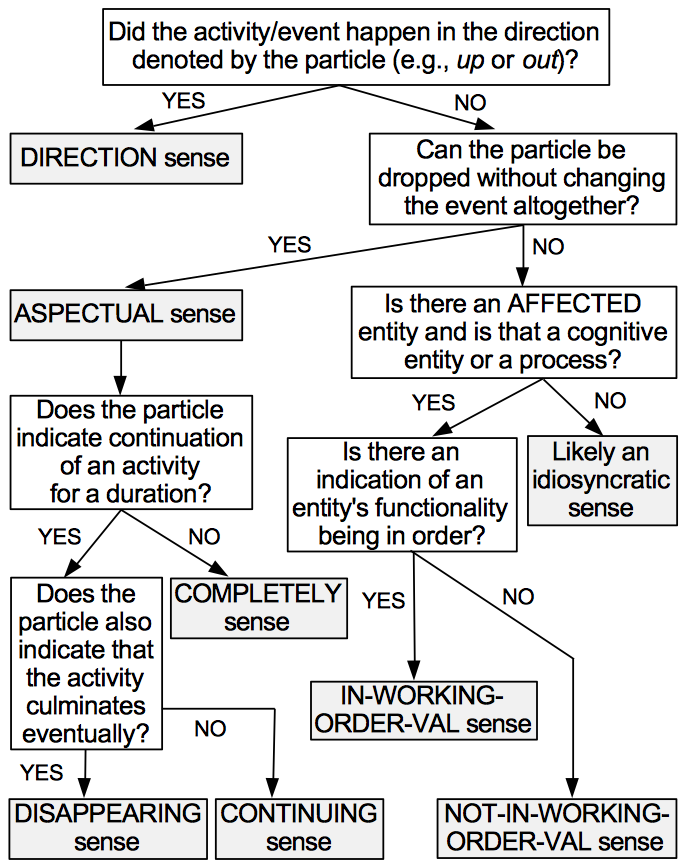
\includegraphics[width=.66\textwidth]{figures/block_sense_uppercase}
%\vspace*{-2mm}
\caption{Tests to identify particle senses}\label{fig:tests-senses}
\end{figure}


\section{Computing semantics of sentences with VPCs} \label{sec:generalizations} 
\largerpage
For the task of interpreting sentences\is{parsing!semantic} with VPCs, we first need to determine if the VPC is compositional or not. We use the heuristics mentioned in \sectref{sec:heuristics} to determine the compositionality of a VPC. For the compositional cases, we get the senses for the verb and the particle from the TRIPS ontology and/or WordNet. The senses for the particles as well as relevant linguistic generalizations to identify these senses are encoded in the TRIPS lexicon and ontology. 
In this section, we briefly discuss some of the generalizations encoded in the ontology and demonstrate the process of computing the semantics of sentences containing compositional VPCs using three example sentences involving VPCs with different senses for the particle \ile{up}: \ile{She cleaned up her room}, \ile{She pushed the ball up}, and \ile{The network came up}. The logical forms (LFs) produced for these sentences using the TRIPS parser, a broad coverage deep semantic parser driven by the TRIPS ontology, are presented in \figref{fig:lf1} to \figref{fig:lf3}.
\clearpage 

\begin{figure}
%\vspace*{-1mm}
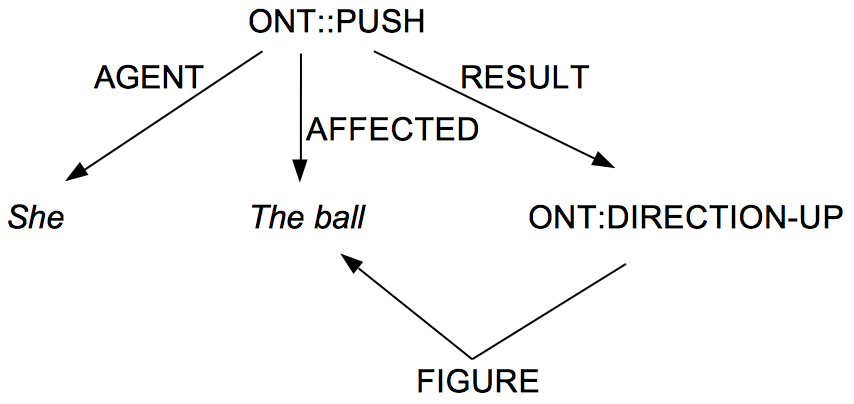
\includegraphics[width=.66\textwidth]{figures/LF1_uppercase}
%\vspace*{-2mm}
\caption{LF for the sentence: \ile{She pushed the ball up.} }\label{fig:lf1}
\end{figure}

\begin{figure}
%\vspace*{-1mm}
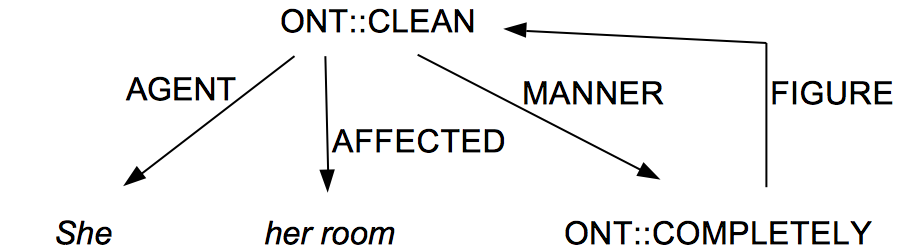
\includegraphics[width=.66\textwidth]{figures/LF2_uppercase}
%\vspace*{-2mm}
\caption{LF for the sentence: \ile{She cleaned up her room.} }\label{fig:lf2}
\end{figure}

\begin{figure}
%\vspace*{-1mm}
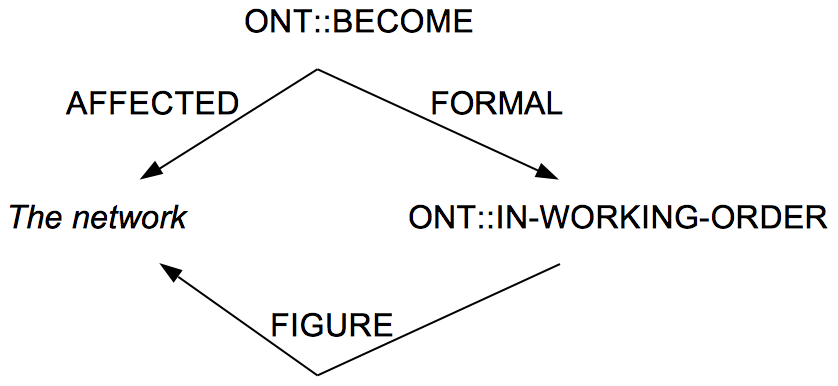
\includegraphics[width=.66\textwidth]{figures/LF3_uppercase}
%\vspace*{-2mm}
\caption{LF for the sentence: \ile{The network came up.}}\label{fig:lf3}
\end{figure}


Particles in compositional VPCs can express the senses mentioned in Tables \ref{tab:1:senseclasses-prtcls}--\ref{tab:1:findings-prtcls-3senses}, and in \figref{fig:tests-senses}. This information is encoded in the TRIPS ontology by adding the ontology types corresponding to these senses in the particle's lexicon. For example, the lexical entry for the particle \ile{up} lists sense ontology types ONT::DIRECTION-UP, ONT::COMPLETELY, and ONT::IN-WORKING-ORDER-VAL, used in \figref{fig:lf1} to \figref{fig:lf3} respectively, among other possible senses.\footnote{For a better idea of what information the lexical entries and semantic/ontology classes carry in the TRIPS lexicon and ontology, see  \url{http://www.cs.rochester.edu/research/cisd/projects/trips/lexicon/browse-ont-lex-ajax.html}.} WordNet sense keys corresponding to the particle may be added in the ontology entries for these sense ontology types. For example, WordNet sense keys up\%4:02:00 and up\%4:02:05 are added in the entry for the sense ontology type ONT::DIRECTION-UP.

The senses that particles express in a VPC may depend on the verb type they combine with in the VPC. That is, a particle may convey the same sense when it appears with any of the verbs in a specific verb ontology class.\footnote{We find that different verb ontology types that were distinguished for other reasons in the TRIPS  ontology \citep{All07} also line up with the particle distinctions.} For example, particles tend to get DIRECTION sense with verbs of motion and CONTINUING sense with atelic verbs that have extended durations (e.g., activity type verbs). With verb ontology types corresponding to continuous-change verbs (which appear under change verbs in the TRIPS ontology), particles tend to get the COMPLETELY sense. Specific verb ontology classes are also identified for specific particles, e.g., particle \ile{down} exhibits COMPLETELY sense with the verbs in the TRIPS ontology class ONT::PURSUE, as can be seen in \ile{The internet \textbf{tracked down} this guy's stolen car (...)}
and \ile{A motorist \textbf{chased down}, slapped, and threatened a boy (...)}.

In addition, we observed an interesting fact that the particles \ile{up} and \ile{out} seem to be in complementary distribution with respect to various verb ontology classes for the COMPLETELY sense. That is, for the COMPLETELY sense, either \ile{up} or \ile{out} is used, but not both with verbs from a specific verb ontology class.\footnote{This observation about the complementary distribution of usage between \ile{up} and \ile{out} may not be accidental. The Law of Differentiation \citep{Pau90,Bre00}, and the Avoid Synonymy principle \citep{Kip83,Cla87} have been proposed in the lexico-semantic sphere which suggest that languages prefer not to have a given semantic slot be filled by two distinct lexical items.} For example, with the verb ontology class ONT::ACQUIRE, \ile{up} is used with COMPLETELY sense, \ile{out} cannot be used with the verbs in this ontology class with the same sense. Note the COMPLETELY sense in the VPC \ile{acquire up} in \ile{Techstars has \textbf{acquired up} Global}, but we do not observe a VPC \ile{acquire out} with the same sense. Similarly, with the verb ontology class ONT::EVOKE-TIREDNESS, \ile{out} is used with the COMPLETELY sense, but \ile{up} cannot be used. Note that we can say, \ile{Someone's a bit \textbf{tuckered out}}, but not \ile{\textbf{tuckered up}}.

Similarly there are generalizations observed for specific senses of particles corresponding to the semantic relation labels. For example, the verb takes a particle with an ASPECTUAL sense as its MANNER argument and the ASPECTUAL sense particle takes the verb as a FIGURE, as is observed in the LF in \figref{fig:lf2}. For the DIRECTION sense class particles, the verb assigns a RESULT argument role instead of a MANNER role to the particle, as illustrated in \figref{fig:lf1}. The particle, on the other hand, assigns the FIGURE role to the AFFECTED entity as in \figref{fig:lf1}. For the IN-WORKING-ORDER-VAL sense% also
, the particle takes the AFFECTED or NEUTRAL entity as its FIGURE argument as is illustrated in \figref{fig:lf3}. Thus, we see that different semantic relations may be involved in sentences with different senses for the particles.

In order to get the correct semantic relations in different cases, we encode this information in the ontology. The sense ontology type ONT::COMPLETELY, used in \figref{fig:lf2}, for example, specifies for its FIGURE argument all the verb ontology types with which a particle gets this sense. This information is presented in %the Verb onttype column and 
the Generalizations column in \tabref{tab:1:findings-prtcls-sense-classes}. Note that %here 
under ONT::COMPLETELY, we list all the verb ontology types with which we get the COMPLETELY sense irrespective of the specific particles used.%with which we get the sense.
\footnote{Note that since the ontology is hierarchical, there is no need to list all the children ontology types as well if the parent ontology types are included.} Hence, ONT::COMPLETELY would specify for its FIGURE argument the ontology types ONT::PURSUE, ONT::ACQUIRE as well as ONT::EVOKE-TIREDNESS, for example. 

Each of the verb ontology types mentioned above specifies which particles can take a specific semantic relation label. For example, the verb ontology type ONT::PURSUE would specify for its MANNER argument particle \ile{down}, verb ontology type ONT::ACQUIRE would specify particle \ile{up}, and verb ontology type ONT:EVOKE-TIREDNESS would specify particle \ile{out}.  

For the DIRECTION senses\is{particle sense classes!direction}, the particle could be replaced with a RESULT-Pre\-po\-si\-tional Phrase (RESULT-PP) in the sentence. For example, the particle \ile{off} in \ile{The officer got \textbf{off} when he spotted an illegally parked car} can be replaced with a RESULT-PP \ile{off his motorcycle} as in \ile{The officer got \textbf{off his motorcycle} when he spotted an illegally parked car}.

Depending on the compliance or violations of constraints such as the ones described above, the parser assigns scores for various parse options involving various senses of the particle in a VPC. The parse with the highest score is selected as the semantic representation of the sentence involving the VPC.

% In the sentence
In \ile{She cleaned up her room} (\figref{fig:lf2}), the verb \ile{clean} (ONT::CLEAN which appears under ONT::CHANGE-STATE in the ontology) is not among the list of relevant verb ontology types with which a DIRECTION-UP sense is licensed for the particle \ile{up}. Additionally, a restriction on the verb argument for the DIRECTION-UP sense is that the argument have a semantic feature [+moveable] which is also violated in the given sentence, since \ile{the room} is generally not a moveable entity. Hence, the parser assigns a low score to the parse which involves the DIRECTION-UP sense for the particle \ile{up} in this sentence. The verb \ile{push}, however, in the sentence in \figref{fig:lf1}, is a movement-related verb and the affected entity \ile{ball} is a moveable object. Hence, the parser assigns a higher score to the parse that involves the DIRECTION-UP sense for the particle \ile{up} in this sentence.

The IN-WORKING-ORDER-VAL sense requires restrictions on the verbs that they take cognitive entities, devices or processes as their AFFECTED arguments which provide service, i.e., they have some functionality associated with them. The AFFECTED argument for the verb \ile{clean}, namely \ile{the room}, in \figref{fig:lf2} does not satisfy this restriction. Similarly, The AFFECTED argument for the verb \ile{push}, namely \ile{the ball}, in \figref{fig:lf1} does not satisfy this restriction. Hence, the parser assigns a low score for the parses involving an IN-WORKING-ORDER-VAL sense for the particle \ile{up} in the two sentences. On the other hand, the entity \ile{The network} in the sentence in \figref{fig:lf3} satisfies the restriction and hence the sentence in \figref{fig:lf3} gets a higher score for the parse that contains IN-WORKING-ORDER-VAL sense for the particle \ile{up}. 

The constraints for the COMPLETELY sense\is{particle sense classes!completely} of the particle \ile{up} are satisfied for the sentence in \figref{fig:lf2}. The verb \ile{clean} is among the set of verbs in the ontology type (ONT::CHANGE-STATE) with which the relevant particle has been identified in the ontology to get this sense. Hence, the parser assigns a higher score to the parse for the sentence with the COMPLETELY sense for the particle \ile{up}. The other two sentences get a lower score for a parse with the COMPLETELY sense for the particle \ile{up}.

Thus, as mentioned above, the parse with the highest score is selected as a semantic representation for each of the sentences involving the VPC. Hence, the sentence in \figref{fig:lf1} has the DIRECTION-UP sense for the particle \ile{up}, the sentence in \figref{fig:lf2} has the COMPLETELY sense, and the sentence in \figref{fig:lf3} has the IN-WORKING-ORDER-VAL sense for the particle \ile{up}.

\section{Conclusion } \label{bha:sec:conclusions}
Identification of MWEs, such as verb-particle constructions, as well as the computation of their meaning is necessary for a broad coverage understanding. It is not plausible to hand enumerate all the possible combinations, although WordNet is an admirable start.  We have described an approach where the meaning of a wide range of VPCs is computed compositionally, with the advantage that VPCs not explicitly found in the lexicon can be both identified and semantically interpreted. To accomplish this, we identified the core senses of particles that have broad application across verb classes. This information is used while building computational lexica. We encoded the generalizations corresponding to various senses of particles in the TRIPS ontology and used them to identify these senses. We found that the generalizations corresponding to grammatical/semantic/ontological information help us identify appropriate senses of the particle. The procedure adopted enables compositional parsing by helping differentiate between particle senses, which is then used to obtain full semantic representations of sentences.

While we have outlined our approach to compute the semantics of sentences with VPCs in English using resources such as the TRIPS lexicon and ontology and WordNet, a similar approach can be adopted to incorporate more lexical or other linguistic resources to further improve semantic parsing\is{parsing!semantic} of sentences involving VPCs in English. Also, such an approach can be adopted for semantic parsing of sentences involving other MWEs, as well as for developing semantic parsing capabilities for other languages using the resources available for those languages.  



\section*{Abbreviations}

\begin{tabularx}{.96\textwidth}{ll}
\textsc{lf} & logical form  \\\textsc{lp}-compositional  & light particle compositional  \\
\textsc{lv}-compositional & light verb compositional   \\
\textsc{mwe} & multiword expression  \\
\textsc{result-pp} & \textsc{result}-prepositional phrase  \\
\textsc{vpc} & verb-particle construction \\
\end{tabularx}



{\sloppy
\printbibliography[heading=subbibliography,notkeyword=this]
}
\end{document}

